\chapter{Results and Discussion}

This chapter presents the findings of this work as well as the work that has been done and the challenges incurred and then discusses them in a wider context. The work regarding the configuration will first be evaluated upon its value and its design principles.

%Is this a sensible result representing reality and fulfilling demands in respect to working SHM and FAIR principles?

%Thoughts on data structure flow.





%\section{Metadata structure}

\section{Metadata system}

The Metadata plays a focal role within this work. It does not only just represent the data but is also vital for honoring the FAIR principles and opening this work up for further use. For completeness the parsing and upload will also be mentioned in this section since it all becomes part of the bigger picture. It also works up its way to achieve low coupling of software parts while maintaining high coherence of the metasystem behind, standardizing its single parts. Advertently achieving structured design as proposed by industry norms such as \textcite{stevens_structured_1974}.
For the data provision, a common ground has been found for the upload so that alterations to further processing parts of the cycle don't necessitate a full reupload of the original data. This common ground asserts that original data is uploaded once with the downside that the DAQ configuration may not be fully interpretable at this stage due not being self-describing metadata.

The following step of configuration solves this problem then by collecting and merging available metadata into a common scheme. This step works upon the DAQ metadata that is already uploaded to the skystash and then fuses it with other metadata sources that are locally available to generate a holistically valid metadata set. Notable is that this step will certainly be part of rather constant modification due to SHM configurations that are also provided within this step. Also the metadata schema is far from complete and will be in need of constant expansion to compensate the complex dimensions of Flight Test Data as well as relevant test configuration data that also may be taken into consideration within this step \ref{fig:digecat_data_sources}. Since this step is far less computationally intensive than the parsing process this is considered as an acceptable tradeoff within this process.

\subsection{Results}


%• Config was developed according to the requirements and embedded into the previously existing system • Config for parameter properties in excel • Config merge performed to get one "true" config from DAQ+general config merge • Config for checks has also been implemented in a JSON-format


It has then be shown to be effective to separate metadata into the unmodified DAQ-data and a set of general metadata that provides all other necessary information. Be it for providing helpful details or vital SHM metadata. Fusing both sets of metadata then into a common set firstly elevates reliability of metadata by taking in account the DAQ-metadata. It then also guarantees interoperability and reusability by transforming metadata into a standardized metadata format that allows to be exchanged for the most effective format available since the transformation process takes marginal effort once the data is digitally available and compounded.
It has then also been adhered to the process standard by not inventing another new standard but respecting existing standards to use an excel sheet for configuration purposes. Using this approach and keeping information centralized, a later migration of data will be much facilitated.

Regarding the algorithmic part, the configuration has been created within a JSON-format. Reducing coupling while allowing a more dynamic expansion of the codebase. This makes it easier to implement changes and reduces the points of entry for making changes for creating new routines


\subsection{Discussion}
%• Good results. • Good adherence to the FAIR guiding principles (quick crosscheck)
%• However config editing in excel is pretty pisspoor from a version control standpoint • Has a lot of potential to become quite powerful as simple changes in config-setup don't influence rest of the toolchain • "low coupling --> high cohesion"

Adherence to the FAIR principles should be the main focus. Especially when handling metadata. The developed metadata handling can assert to have guaranteed the findability, interoperability and reusability within the metadata part of this work since the metadata clearly describes the data at hand (Findability), it then also clearly describes what attributes the data has and with which attributes the SHM algorithms will be run (Interoperability, Reusability) to then allow future users to reproduce and comprehend the full SHM process. In addition, the low coupling and high cohesion are central paradigms of this work.

The current form of the general config however poses some serious challenges and issues. It has the upside of being centralized but the downside of being in a not version-controlled environment. Not allowing backtracking and making search for faults very difficult. It also hinders development since experimental changes can only be made by copying to a local version that is then not version-controlled. It also does not allow dynamic changes to the metadata and in general does not adhere to the presented FAIR principles. However, once this issue has been fixed this work may bring more than marginal improvements to the world of data quality, allowing small changes of settings in the general configuration to trigger the SHM toolchain, updating data quality indices as you go. This metadata-workflow is also not limited to the  ISTAR data and may be applied to other aircraft or even machines or systems as well since the area of sensors is a constantly growing field. Even considering that in the Internet of Things (IoT) and Internet of Production the actual sensor values are hardly ever checked. Since this is a growing topic this work attempts to lay a solid foundation upon which future endeavors may build upon and flourish.


\section{Algorithms (Interoperable, Reusable)}

The core component of this work are the algorithms to actually detect the errors. These Algorithms have been implemented to catch the major recurring errors that are known to be within the datasets. Although most often errors occur in Level 1 and become critical due to oversight, other error types are also important to consider. The sheer amount of ISTAR sensors voids any ability to maintain an overview over the entire system.

For trial and erroring and embarking on the SHM journey, the experimentally installed sensors in the ISTAR serve as a significantly better benchmark for errors since they are less reliable than the inherent aircraft sensors and thus also produce more interesting errors. Four errors from accelerometers and strain gauges are shown in figure \ref{fig:error_plots}. Ranging from interrupted transmission to odd offsets and plain overflow values.

\begin{figure}[h]
    \centering
    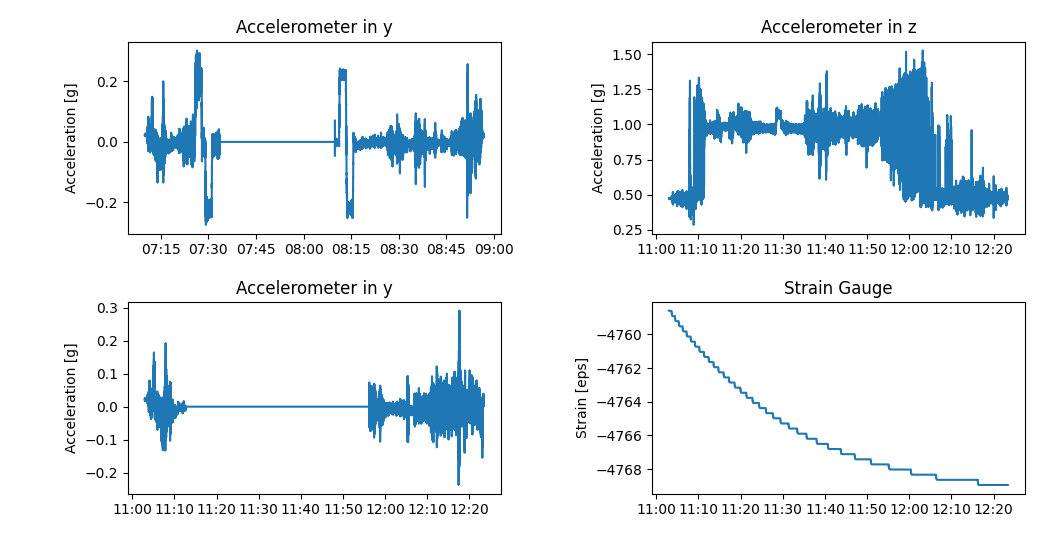
\includegraphics[width=0.8\textwidth]{python_functions/images/error_plots}
    \caption{Exemplary Errors occuring for experimental accelerometers and strain gauges.}
    \label{fig:error_plots}
\end{figure}


\subsection{Results}


In the following, the outcomes of algorithms of Levels 1-3 are presented and henceforth discussed.
The validation errors shown in figure \ref{fig:error_plots} are mostly solved since some strange errors make automatic detection difficult.
Beginning with Level 1, all not parameters that have not made it to the skystash but have been expected to are filtered out. Acknowledging that Level 1 merely builds the first defense against errors this is a good start for the SHM, catching all errors that are plainly not available.

In Level 2 the most recurring faults are caught. It evaluates single sensor timeseries and possibly transforms them to then check against the limits defined in the config. In plots \ref{fig:results_050303_spectrogram} the basic spectrogram for the first given accelerometer in \ref{fig:error_plots} is given.
\begin{figure}
    \centering
    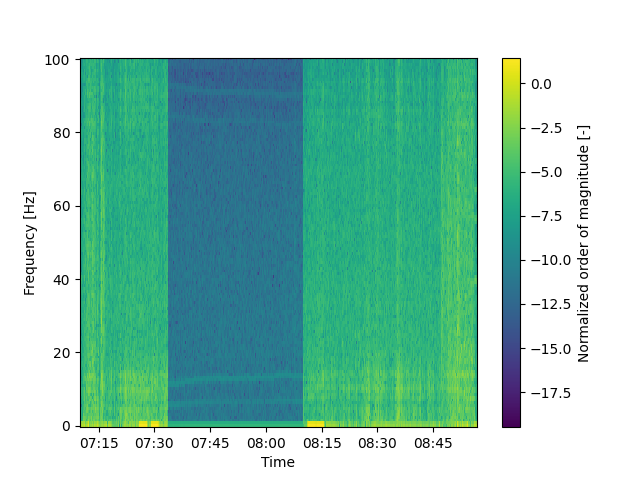
\includegraphics[width=.7\textwidth]{03_figures/python_functions/images/FUS_050303_spectro.png}
    \label{fig:results_050303_spectrogram}
    \caption{Spectrogram analysis of the erroneous accelerometer}
\end{figure}
Based upon this spectrographic analysis outliers can be identified whose movement is either too high or too low. Using this spectrogram an averaged normed amplitude value can be calculated that represents the sensor movement. In figure \ref{fig:results_050303_1} as well as \ref{fig:results_050303_2} the erroneous behaviors are clearly identified by falling outside the amplitude boundaries that have previously been defined in the general configuration.
Additional faults such as the strain gauge forming the bottom right value in figure \ref{fig:error_plots} can quickly be identified since a regular value of such a sensor generally falls into the limits of $[-1000, +1000]$. This becomes obvious in figure \ref{fig:results_230306} when comparing to the limits in red.
\begin{figure}
    \centering
    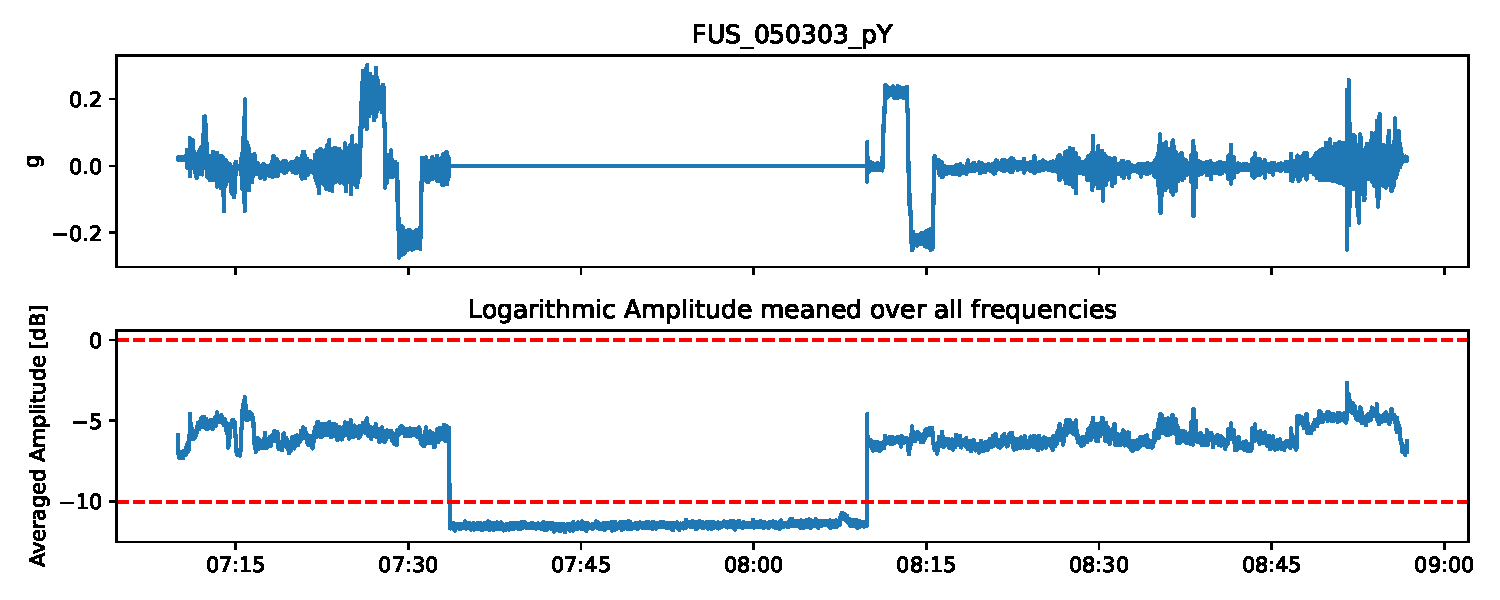
\includegraphics[width=\textwidth]{03_figures/python_functions/images/FUS_050303}
    \label{fig:results_050303_1}
    \caption{Original Signal over STFT Averaged Amplitude}
\end{figure}
\begin{figure}
    \centering
    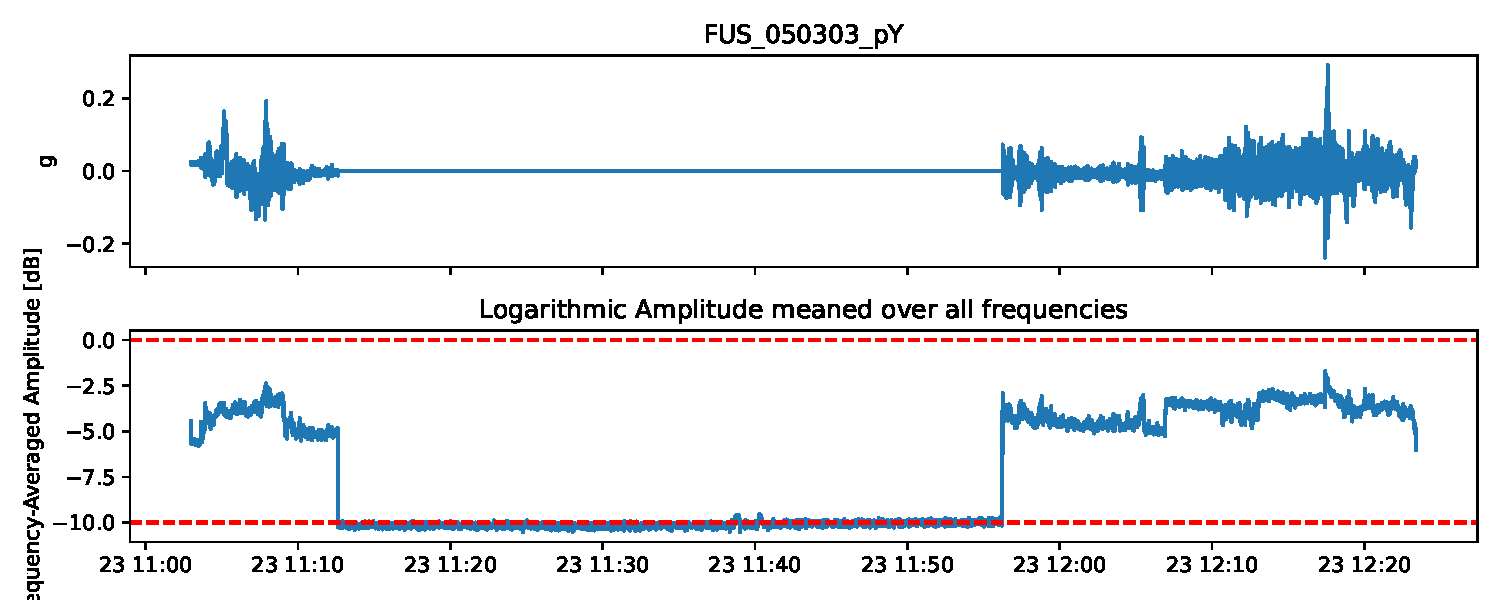
\includegraphics[width=\textwidth]{03_figures/python_functions/images/FUS_050303_2}
    \label{fig:results_050303_2}
    \caption{Original Signal over STFT Averaged Amplitude}
\end{figure}
\begin{figure}
    \centering
    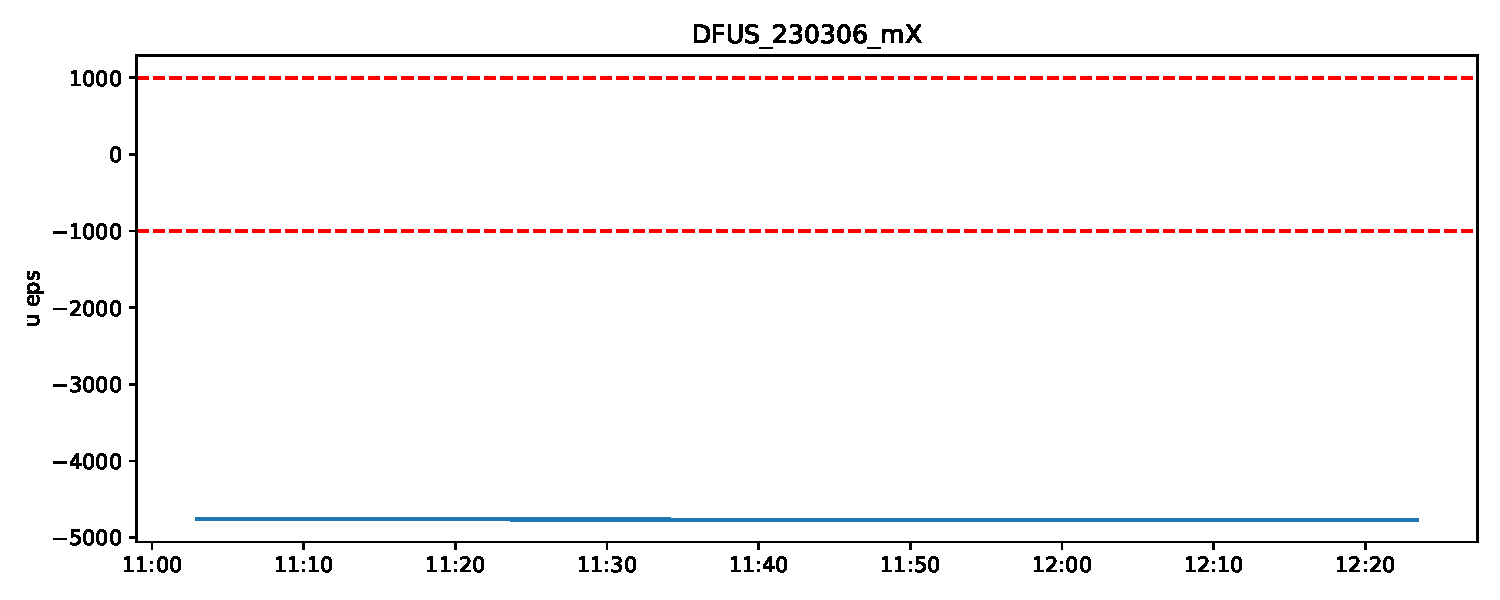
\includegraphics[width=\textwidth]{python_functions/images/DFUS_230306}
    \caption{Malfunction of the Strain Gauge}
    \label{fig:results_230306}
\end{figure}

Detecting smaller, constant offsets that are within limits such as the accelerometer in z direction in the top right plot in figure \ref{fig:error_plots} does not get filtered by Level 2 algorithms as shown in figure \ref{fig:results_050209}.
\begin{figure}
    \centering
    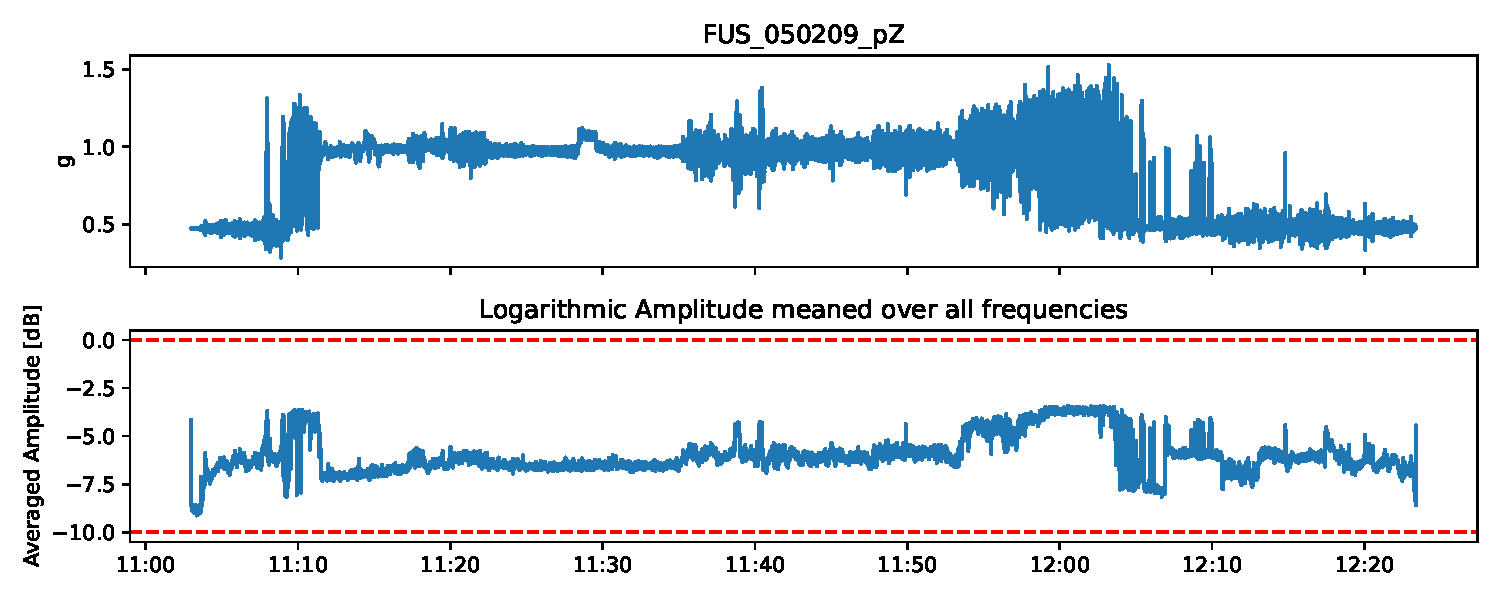
\includegraphics[width=\textwidth]{03_figures/python_functions/images/FUS_050209}
    \label{fig:results_050209}
    \caption{Analysis of the offset vertical accelerometer}
\end{figure}

To detect an offset in z direction it is more sensible to include other correlating z sensors or the rigid body model of the aircraft. Determining in acceleration in z direction within such a model should allow correlation of flight angles as well as other accelerometers in the Inertial Measurement Units (IMUs) as well as relational angles indicating turning of the aircraft and hence more acceleration in z-direction.
\begin{figure}
    \centering
    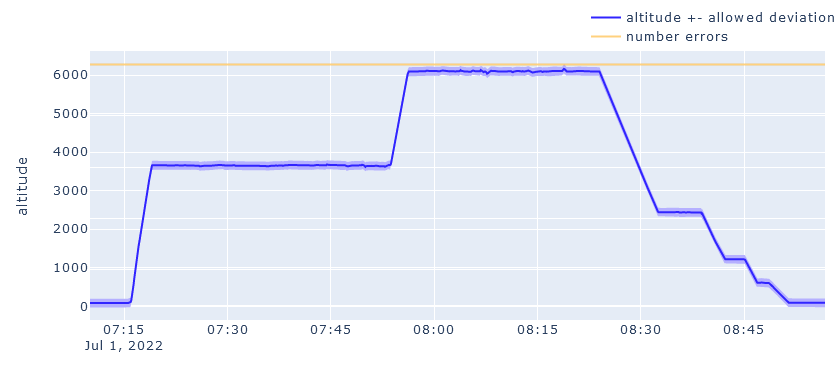
\includegraphics[width=0.9\textwidth]{stashboard_level3_zoomed}
    \caption{Level 3 calculation for barometric altitudes with a tolerance area (transparent blue)}
    \label{fig:stashboard_level3_zoomed}
\end{figure}

For now, however, only the altitude with the specialization of the barometric altitudes has been implemented. In Level 3 an automatic limit gets calculated based on the fused signal. Here, the fused signal gets detrended to remove any trends and the standard deviation of the signal gets used to measure expected deviations. The fused signal combined with the expected deviation is shown in Stashboard figure \ref{fig:stashboard_level3_zoomed}.

Additionally, level 3 serves as an additional layer of safety against errors. Acting in accordance to the swiss cheese model of secure, redundant system. It also is possible to detect errors with a higher precision compared to the Level 2 algorithms.

%todo: show highpassfiltering and signal extraction



\paragraph{Choosing check parameters}

Automatically setting boundaries for Level 2 has proven to difficult due to the sheer difference of sensor behavior available. Hence, the automatically set limits for Level 2 were abandoned and replaced by hard limits that needed to be set in the general config. However, automatically determined boundaries were still employed and shown to be working for Level 3. Using the detrended signal has proven to deliver sensible limits as shown in the Stashboard in figure \ref{fig:stashboard_level3}.

However, setting limits for Level 2 still requires some trial and error to reliably work for sensors with the validation loop being driven by previously detected error types. It shows that while conservatively chosen ranges do not indicate many occurrences, tighter limits enable more detailed monitoring. Choosing a range still need some tuning since the limits at figure \ref{fig:results_050303_1} seem safe but for figure \ref{fig:results_050303_2} seem very close to detection. Thus, still needing further investigation to safely predict errors. Possibly implementing other type of sensor movement analyzes to deliver results that are more reliably and more tailored to various sensor.

Another interpretation of the sensitivity in analysis methods lies in too tight tolerances. These may detect every small aberration but generate too many occurrences when actual malfunctions are of interest and not every single perturbation.



\paragraph{Data Sampling}
Some Oversampling of sensors happens in the DAQ due to the aircraft systems.
The ASCB bus samples all parameters to 20Hz and consequentially data gets either lost or needlessly oversampled in the process. This makes potentially noisy sensors output the same value twice in a row since the DAQ hasn't yet received the new sensor data and outputs the same value multiple times in a row. Even sensors with a high noise ratio such as the fine part of a GNSS latitude signal outputs the same value twice in a row which is highly unlikely to happen on a statistical basis. Since this occurs quite often the question arises if the actual sampling may be lower than the actual data. Perhaps justifying resampling at certain process to mitigate the changes made by the systems between sensor and DAQ.



\subsection{Discussion}
The results from the algorithms speak for themselves. Although the entire configuration set is not complete and the system is in prototype stadium good results have been achieved. Most of the required errors and malfunctions have been identified by the SHM developed in this work and even if these algorithms may not suffice more complex errors, the overall architecture makes integration of new algorithms for quick deployment easy.

The results in Level 1 are primarily satisfying the application's needs. However, additional interfaces could be implemented displaying sensor subsets in a hierarchical view similar to Level 3 Stashboard implementation (see figure \ref{fig:stashboard_level3}). This could facilitate interpretation which subset of experiments is currently performed. E.g. whether the Nose boom of the ISTAR is presently used based on the given data and metadata.

Level 2 algorithms worked well on the posed problems and also detected complex errors such as the accelerometer faults that resulted in a very little amount of noise. Using Level 2 approaches enabled detection of most known errors, providing a substantial foundation for the proceeding work on ISTAR data. Implementing new functions is realized by using pandas series and dataframes for function in- and outputs and modifying the SHM JSON-configuration.
The FMEA developed also paves the way for further advancements such as a real-time implementation that may be used during experiments to detect possible sensor malfunctions based on processes that are computationally frugal and are able to run in real-time.

Parity Equations enable correlation of parameter behavior even though they present a prototypical beginning for FMEA implementations in the SHM. Neglecting the limitations of Parity Equations they still provide value and truth for correlation making them indispensable in their function as white-box models. The Parity Equations developed in this work still has potential. It may be developed further to include a rigid body model of the aircraft, correlating various axes and states to finally achieve a minimal model error.
Applications in other fields might also find this approach useful. Since the configuration has the only constraint of being hierarchical other physical relations such as in industrial applications can also be represented once these physical relations are mapped to python functions.
Considering further possibilities for Level 3 FMEA various approaches could be assessed and implemented. These would be methods such as Kalman Filtering \cite{lie_synthetic_2013}, PCA \cite{isermann_fault-diagnosis_2006} and other analytical approaches \cite{freeman_air_2013, perhinschi_integrated_2010}.  Exceeding the conventional FMEAs presented in figure \ref{fig:FMEA-methods}, novel methods ranging from model driven designs such as the Pseudo Transfer Function approach \cite{aljanaideh_aircraft_2015} up to state of the art data-driven models for image processing such as GANomaly \cite{akcay_ganomaly_2018} could be implemented. These could be modified for use in research data using latent spaces to identify principal state parameters as well as identifying possibly new hidden correlations.

Within the algorithmic step it has been endeavored to comply with the Interoperable and Reusable criteria of the FAIR principles. Implementing this by using JSON-configurations in standardized formats when possible and decoupling the actual algorithmic from the data communication by using pandas as the interface for the python functions.

\section{Visualization (Accessible, Interoperable, Reusable)}
An interactive frontend for the data quality report has been developed to enable Accessibility of the SHM. Visualizing the data quality for an entire flight dataset at a single glance. Searchable metadata tags enable a dynamic search within the skystash database and due to its web based architecture in dash it can be deployed as a webservice to facilitate usage. It is, however, far from complete and still needs optimization.

\subsection{Results}
As mentioned in \ref{chap:4-visualization}, the Stashboard allows rapid SHM prototyping and quickly generates an overview over ISTAR flights' data quality, swiftly summarizing the large datasets. It interfaces with the skystash over its python Application Programming Interface (API) and using the JSON-report data it is an extension module to provide a Human-Machine Interface (HMI) for the SHM.

The Timeline graph serves as a starting point to detect sensor failures that are associated with sensors outputting invalid values and thus having strange start- and end-times of their respective measurement. An advantage of this display is that it works out of the box on all skystash flights  since it accesses automatically generated skystash data, not needing any processing and SHM.

The Level 1 implementation currently is available in the shape of a gauge, indicating the percentage of available sensors. A helpful addition for later work could be the aforementioned visualization of sensor groups in hierarchical overview. Perhaps color mapping single sensors and sensor groups to their availability or other relevant properties.

For level 2, any algorithms may be dynamically added to the existing configurations in the data processing step. Integrating this works without troubles since the JSON-report allows dynamic extensions on level 2 attributes.
In Level 3, it has been achieved to compare similar sensors that represent the same state variables by representing sensor relations within a tree-structure, the fused signal of all sensors with its automatically detected limit and overall sensor offsets to detect any strong biases of sensors.

\subsection{Discussion}

This dashboard implements a quick overview and architecturally attempts a low coupling high coherency to the skystash and the other parts of the SHM-toolchain, having the skystash API serve as the only interface needed to operate the Stashboard.
Regarding FAIR guidelines, this step fulfills the Interoperability step, allowing any flight with a SHM-report to be loaded and displayed, lowering the barrier of entry for entering the world of data quality. Findability of data is then additionally guaranteed by providing a tool to check any dataset for its inherent data quality, facilitating data discovery by contributing a new method to clearly interpret data quality.
For future expanses, new data quality visualizations and overall displays allow to be implemented in the dashboard structure. Also necessary to maintain overview would be aircraft landing page superset of the current dashboard. This method then may give a better overview over the entire aircraft lifespan and the reliability of its employed sensors and their failure rates. Additional implementations may add various analytic tools for the Flight Test Instrumentation Group to further analyze data such as the TerraWarn-Program, currently being developed at the FTI-group, analyzing flight performances for internal debriefing purposes. Other methods could be a Flight Data Player that allowed to replay the flight at any moment, generating data-quality analyzes for that specific point in time. Overall, this work provides a fundamental base for further skystash analytic tooling in the Digital Twin project, honoring the FAIR guidelines.


\section{Integration of the application}

Summarizing the development, the integration into the skystash ecosystem builds the foundation for a novel data space for Flight Test Data. Following figure \ref{fig:fti_microservices}, all tools are dependent on the skystash and serve as extensions for the existing architecture, expanding it to elevate data interpretability which is vital in the jumble of Research Data available. The programming standard of low coupling but high cohesion \cite{stevens_structured_1974} leverages the skystash API and allows for reduction of technical debt in the future, making maintenance and expansions on single components less complex, reducing interactions.
The overall evaluation of FAIR principles is shown in figure \ref{fig:FAIR_evaluation}. Starting from the upload to the skystash. The genuine DAQ data and metadata is preserved. Metadata Enrichment then decodes the DAQ config and assigns extended information to the DAQ metadata and enhancing the knowledge further by also adding SHM-configurations. Within the following data processing step, all metadata for calculations is already available and the processing step can run without any interaction and also allowing backtracking based upon the enriched metadata that provides the data processing configuration. Finally, the report is uploaded to the skystash and then as a valuation available which can then get interpreted by the data visualization step which allows quick interpretation of the generated report.


\begin{figure}
    \centering
    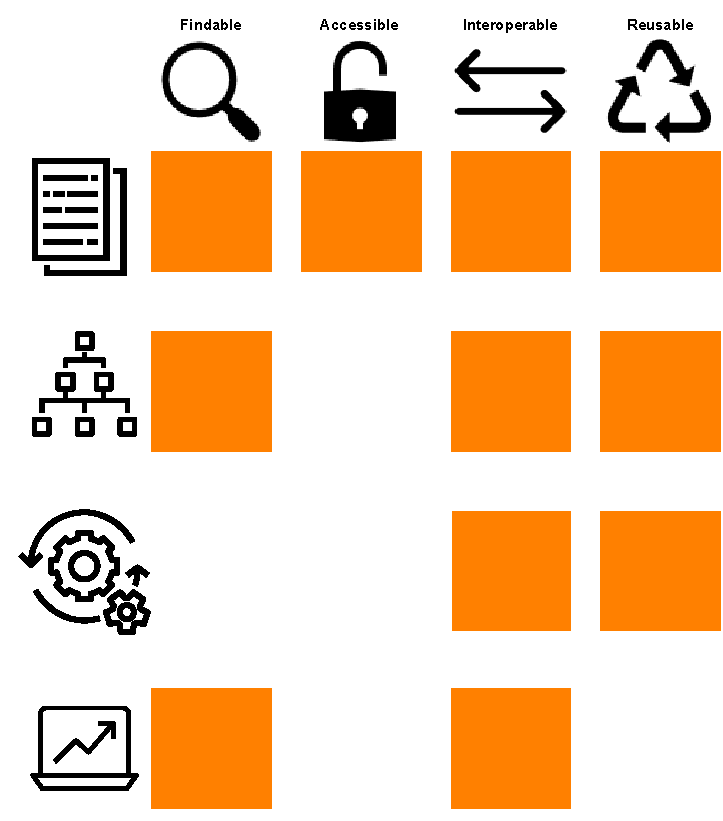
\includegraphics[width = 0.6\textwidth]{FAIR_evaluation}
    \caption{Correlating parts of this work with adherence to the FAIR guiding principles}
    \label{fig:FAIR_evaluation}
\end{figure}

\section{Summary}
The past chapter has shown the outcomes of this work and discussed tradeoffs as well as successes followed by opportunities for expansion which could be realized in future work.
This work delivers a prototype for a Sensor Health Monitoring Infrastructure. It establishes the SHM-process as a holistic toolchain of singular methods to enable future expansion by design.



